% % -*- coding:utf-8 -*-
\documentclass[aspectratio=169,10pt]{beamer}
\nonstopmode

\usepackage{appendixnumberbeamer}
\usepackage{graphicx}
\usepackage{url}
\usepackage{amsmath, amssymb}
\usepackage{pifont} %fuer checkmarks
% color palette
\definecolor{tu01}{HTML}{84B818}
\definecolor{tu02}{HTML}{D18B12}
\definecolor{tu03}{HTML}{1BB5B5}
\definecolor{tu04}{HTML}{F85A3E}
\definecolor{tu05}{HTML}{4B6CFC}
\definecolor{tu06}{HTML}{E3B505}
\definecolor{tu07}{HTML}{AF331D}
\definecolor{tu08}{HTML}{000000}
\definecolor{tu09}{HTML}{AAAAAA}
\definecolor{tu10}{HTML}{444444}
\definecolor{tu11}{HTML}{84B818}

% mixed and light colors
\colorlet{tu01light}{tu01!33}
\colorlet{tu02light}{tu02!33}
\colorlet{tu03light}{tu03!33}
\colorlet{tu04light}{tu04!33}
\colorlet{tu05light}{tu05!33}
\colorlet{tu06light}{tu06!33}
\colorlet{tu07light}{tu07!33}
\colorlet{tu08light}{tu08!33}
\colorlet{tu09light}{tu09!33}
\colorlet{tu10light}{tu10!33}
\colorlet{tu11light}{tu11!33}

\colorlet{tu01midlight}{tu01!50}
\colorlet{tu02midlight}{tu02!50}
\colorlet{tu03midlight}{tu03!50}
\colorlet{tu04midlight}{tu04!50}
\colorlet{tu05midlight}{tu05!50}
\colorlet{tu06midlight}{tu06!50}
\colorlet{tu07midlight}{tu07!50}
\colorlet{tu08midlight}{tu08!50}
\colorlet{tu09midlight}{tu09!50}
\colorlet{tu10midlight}{tu10!50}
\colorlet{tu11midlight}{tu11!50}

\colorlet{tu01dark}{tu01!80!black}
\colorlet{tu02dark}{tu02!80!black}
\colorlet{tu03dark}{tu03!80!black}
\colorlet{tu04dark}{tu04!80!black}
\colorlet{tu05dark}{tu05!80!black}
\colorlet{tu06dark}{tu06!80!black}
\colorlet{tu07dark}{tu07!80!black}
\colorlet{tu08dark}{tu08!80!black}
\colorlet{tu09dark}{tu09!80!black}
\colorlet{tu10dark}{tu10!80!black}
\colorlet{tu11dark}{tu11!80!black}

\colorlet{lightgray}{gray!25}
\colorlet{midlightgray}{gray!50}
\colorlet{anthracite}{black!85}

% aliases
\colorlet{tudo}{tu01}
\colorlet{tuorange}{tu02}
\colorlet{tudolight}{tu01light}

% \usepackage{beamerthememetropolis}
\usetheme[progressbar=frametitle,noslidenumbers]{metropolis}
\newcommand{\themename}{\textbf{\textsc{metropolis}}\xspace}


\usepackage{xcolor}


\title{Abschlusspr\"asentation Projekt 2}
% \subtitle{Learning to Identify Similarities between Mathematical Expressions}
\author{Pouria Araghchi 170468, Kai Lukas Ilmenau 225338, Naveed Niazi 214471}

\institute{TU Dortmund - Fachprojekt zu "Routingalgorithmen"}
\titlegraphic{\hfill
\includegraphics[height=8mm]{tu-do-logo.pdf}}

\date{\today}

\begin{document}

\maketitle
% %%%%%%%%%%%%%%%%%%%%%%%%%%%%%%%%%%%%%%%%%%%%%%%%%%%
% %%%%%%%%%%%%%%%%%%%%%%%%%%%%%%%%%%%%%%%%%%%%%%%%%%%
% Kai
% %%%%%%%%%%%%%%%%%%%%%%%%%%%%%%%%%%%%%%%%%%%%%%%%%%%
% %%%%%%%%%%%%%%%%%%%%%%%%%%%%%%%%%%%%%%%%%%%%%%%%%%%
\section{Kai}

\begin{frame}{Die Topologie}
\begin{columns}
\begin{column}[t]{0.7\paperwidth}
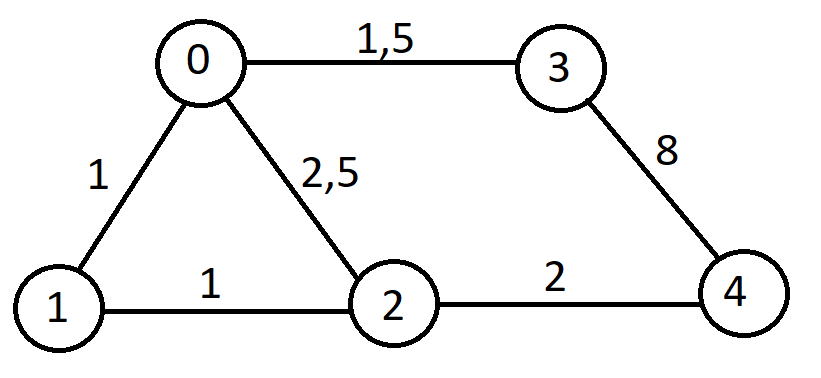
\includegraphics[width=\textwidth]{images/kai1.png}
\end{column}
\begin{column}[t]{0.3\paperwidth}
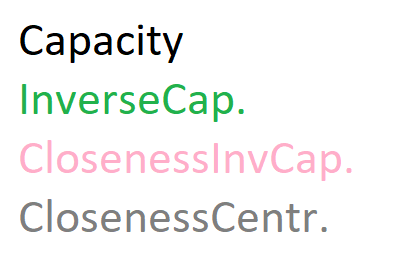
\includegraphics[width=\textwidth]{images/kai_legend.png}
\end{column}
\end{columns}
\end{frame}

\begin{frame}{Inverse Capacity}
\begin{columns}
\begin{column}[t]{0.7\paperwidth}
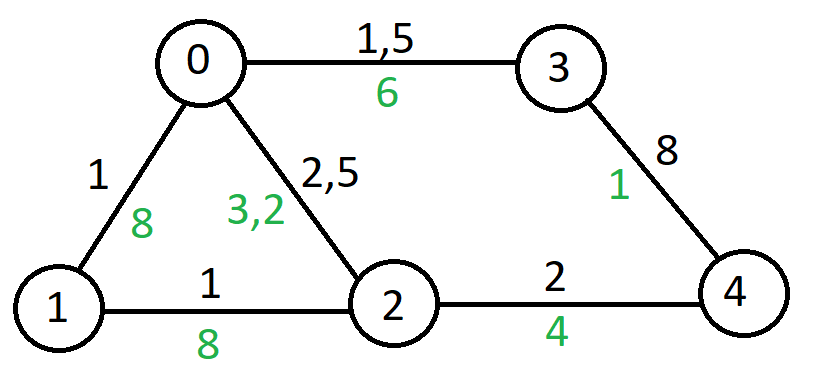
\includegraphics[width=\textwidth]{images/kai2.png}
\end{column}
\begin{column}[t]{0.3\paperwidth}
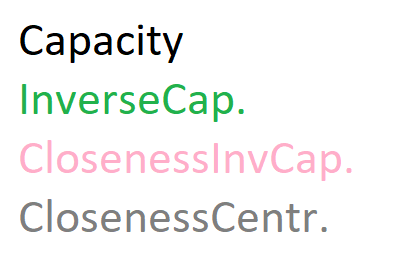
\includegraphics[width=\textwidth]{images/kai_legend.png}
\end{column}
\end{columns}
\end{frame}

\begin{frame}{Closeness Centrality Werte}
\begin{columns}
\begin{column}[t]{0.7\paperwidth}
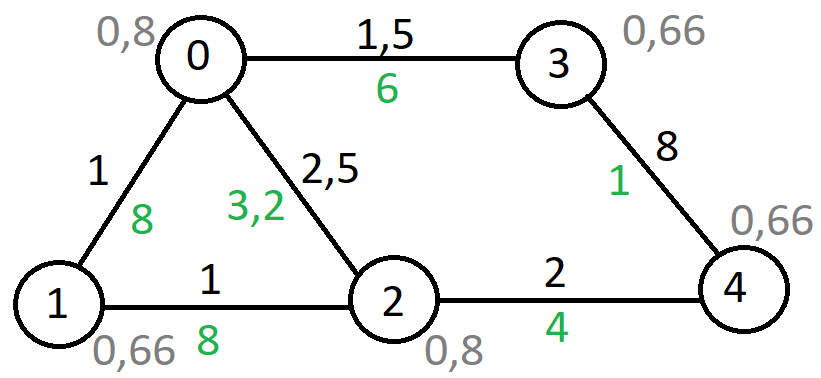
\includegraphics[width=\textwidth]{images/kai3.png}
\end{column}
\begin{column}[t]{0.3\paperwidth}
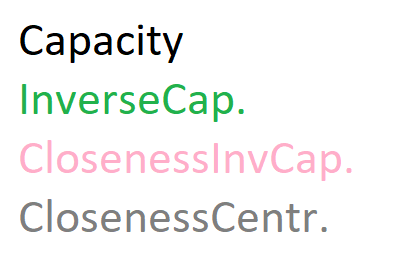
\includegraphics[width=\textwidth]{images/kai_legend.png}
\end{column}
\end{columns}
\end{frame}

\begin{frame}{Closeness Centrality With Inverse Capacity}
\begin{columns}
\begin{column}[t]{0.7\paperwidth}
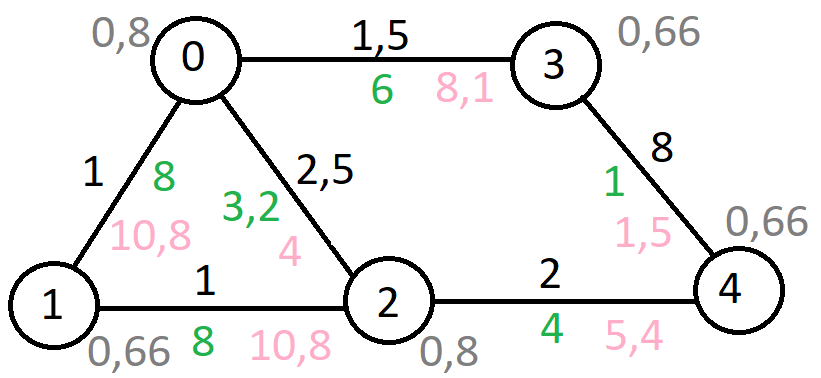
\includegraphics[width=\textwidth]{images/kai4.png}
\end{column}
\begin{column}[t]{0.3\paperwidth}
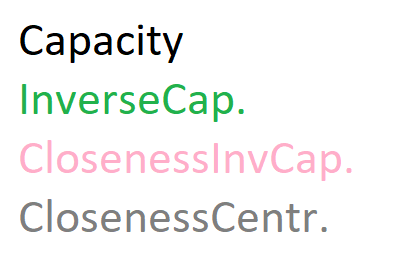
\includegraphics[width=\textwidth]{images/kai_legend.png}
\end{column}
\end{columns}
\end{frame}

\begin{frame}{Mit Demands}
\begin{columns}
\begin{column}[t]{0.7\paperwidth}
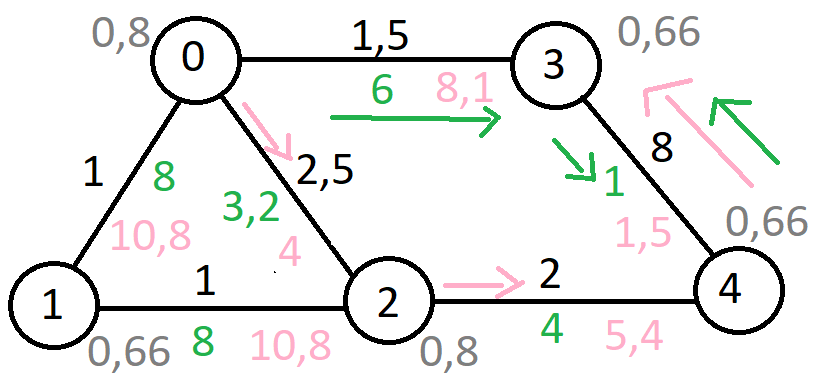
\includegraphics[width=\textwidth]{images/kai5.png}
\Large
Demands von 0 nach 4 (eine Capacity-Einheit) und von 4 nach 3 (acht Capacity-Einheiten)
\end{column}
\begin{column}[t]{0.3\paperwidth}
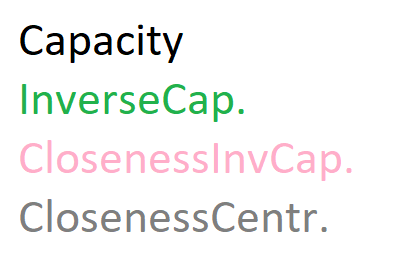
\includegraphics[width=\textwidth]{images/kai_legend.png}
\end{column}
\end{columns}
\end{frame}

\begin{frame}{Boxplots}
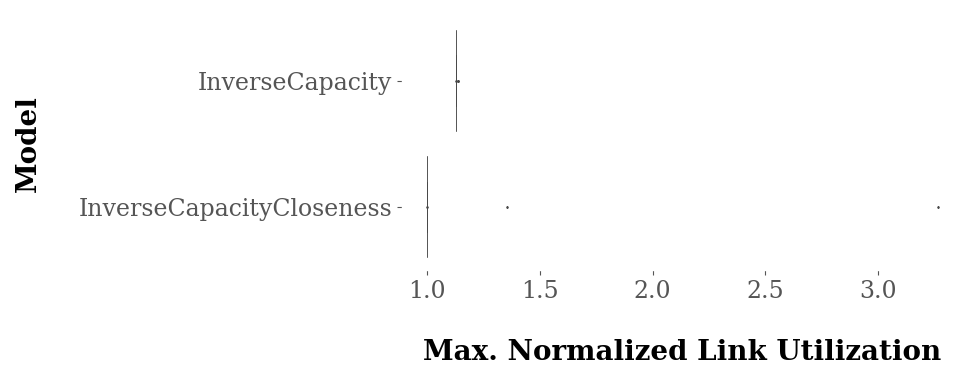
\includegraphics[width=\textwidth]{images/kai6.png}
\end{frame}

\begin{frame}{Ist meine Algorighmus besser?}
\Large
\begin{itemize}
    \item in diesem speziellen Setting: Ja
    \item "designed" Topologie\newline
    $\rightarrow$ lange Suche nach guter Topologie f\"ur den Algorithmus
    \item Siehe Projekt 1: $Inverse\_Capacity$ im Durchschnitt besser als meine Anpassung
\end{itemize}
\end{frame}
% %%%%%%%%%%%%%%%%%%%%%%%%%%%%%%%%%%%%%%%%%%%%%%%%%%%
% %%%%%%%%%%%%%%%%%%%%%%%%%%%%%%%%%%%%%%%%%%%%%%%%%%%
% Naveed
% %%%%%%%%%%%%%%%%%%%%%%%%%%%%%%%%%%%%%%%%%%%%%%%%%%%
% %%%%%%%%%%%%%%%%%%%%%%%%%%%%%%%%%%%%%%%%%%%%%%%%%%%
\section{Naveed}
\begin{frame}[fragile]{}
\begin{center}
    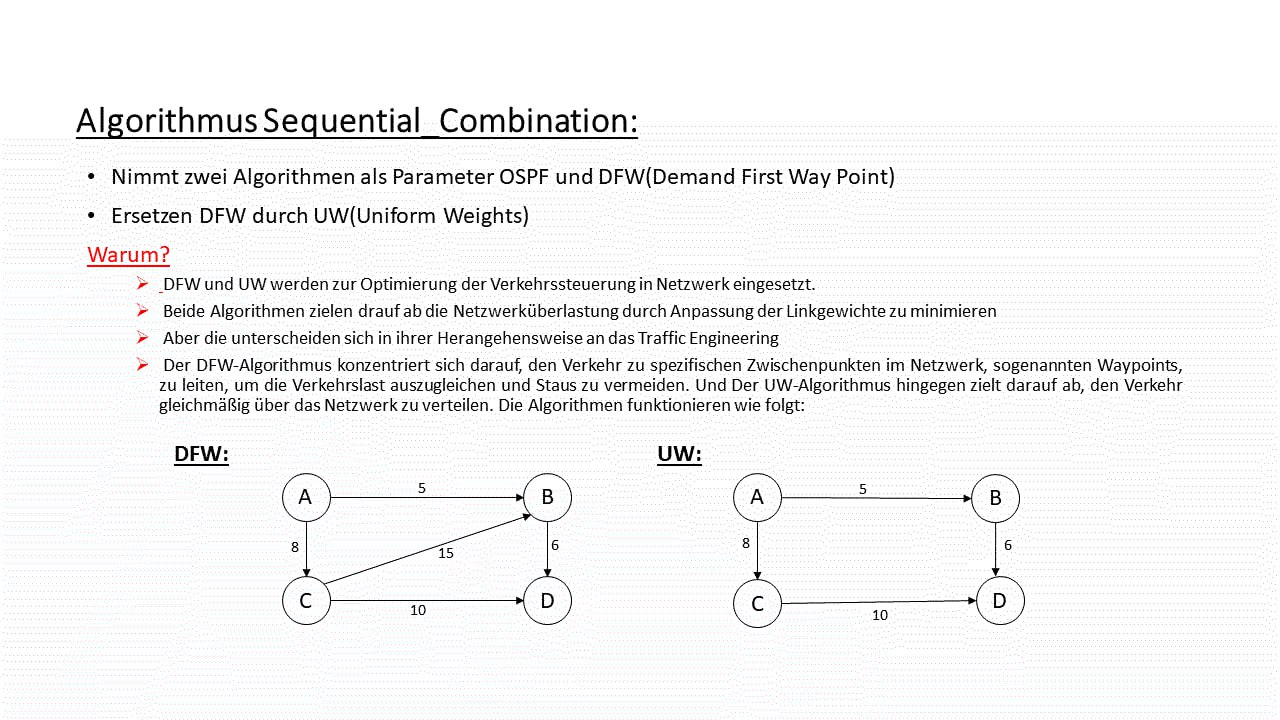
\includegraphics[width=\textwidth]{images/naveed_7.jpg}
\end{center}
\end{frame}
\begin{frame}{Ergebnisse}
\begin{center}
    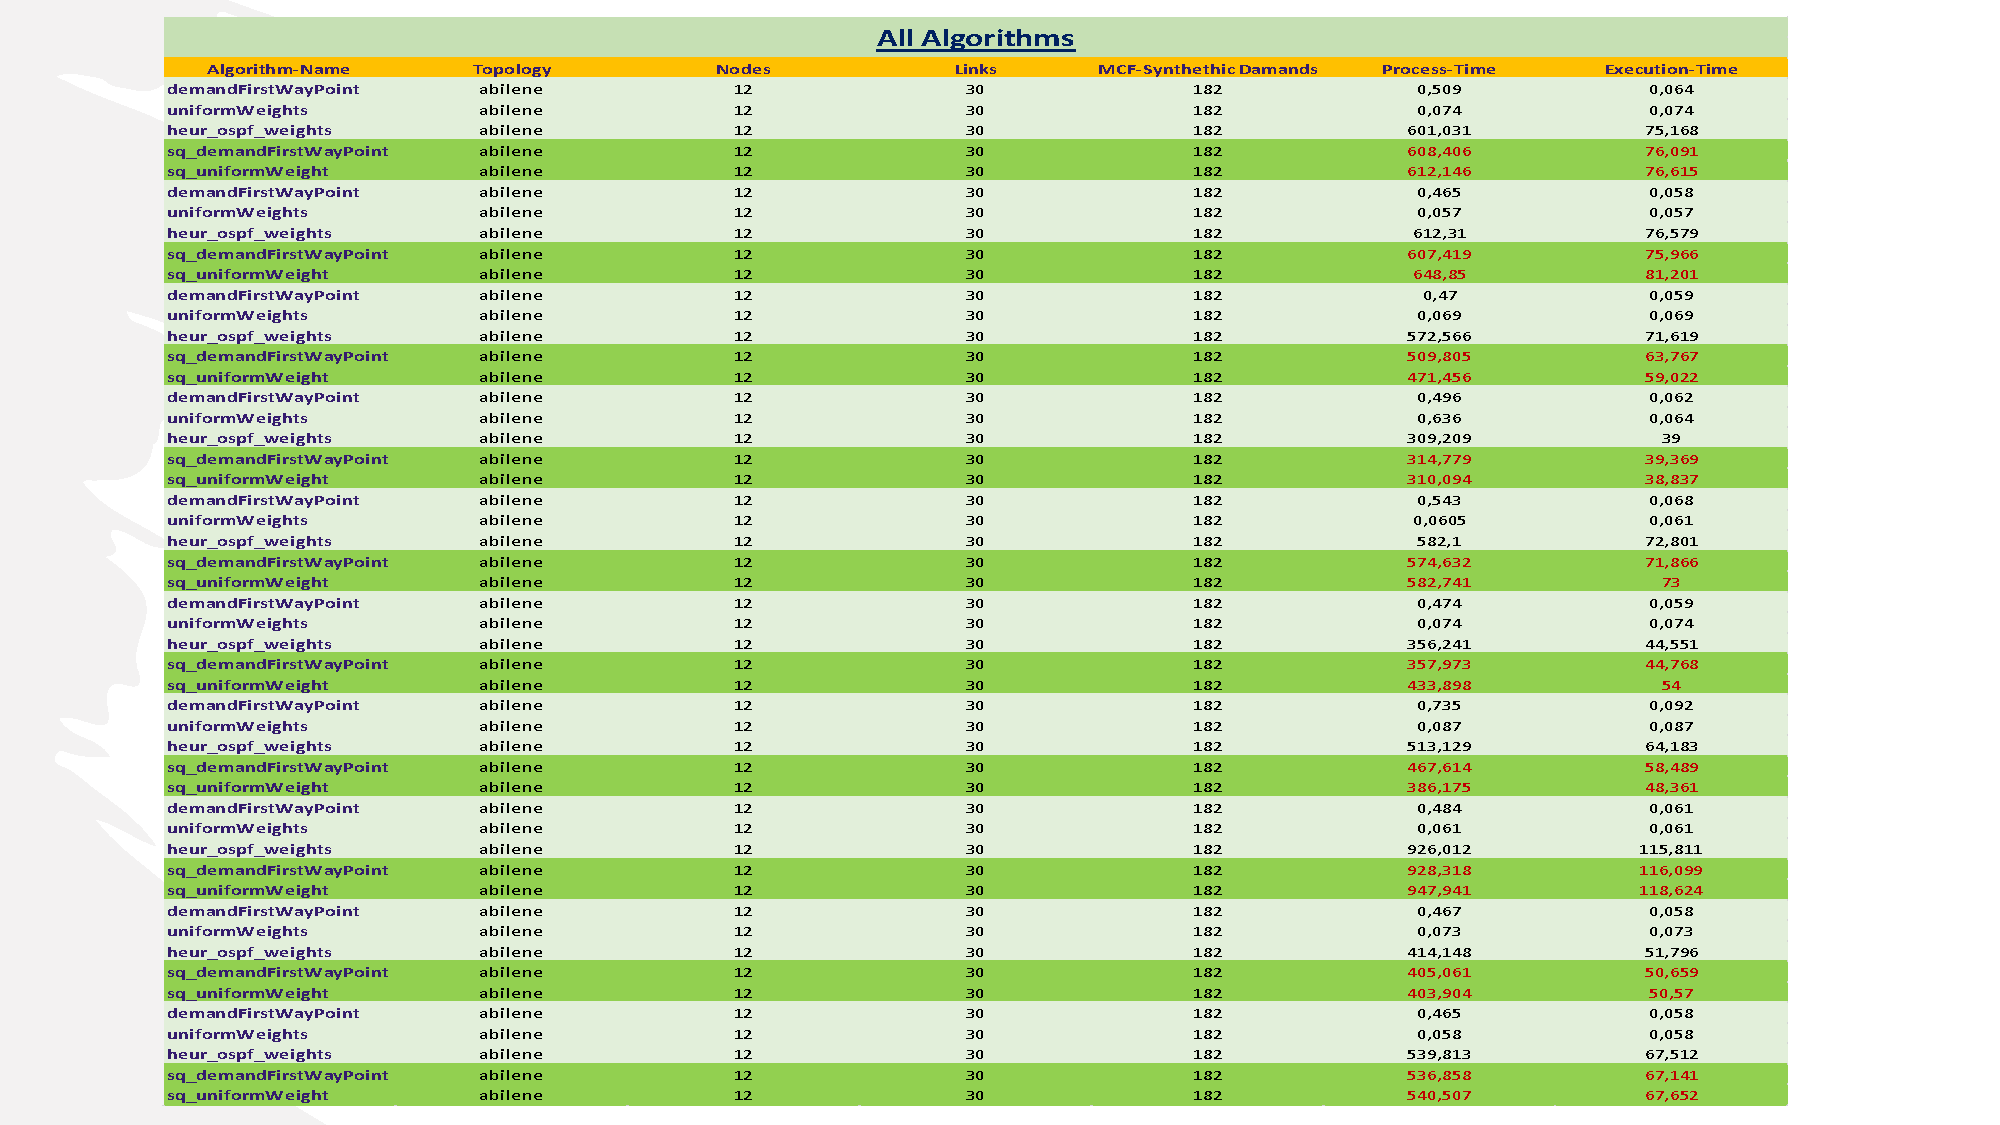
\includegraphics[width=\textwidth]{images/naveed_11.pdf}
\end{center}
\end{frame}
\begin{frame}{Ergebnisse}
\begin{center}
    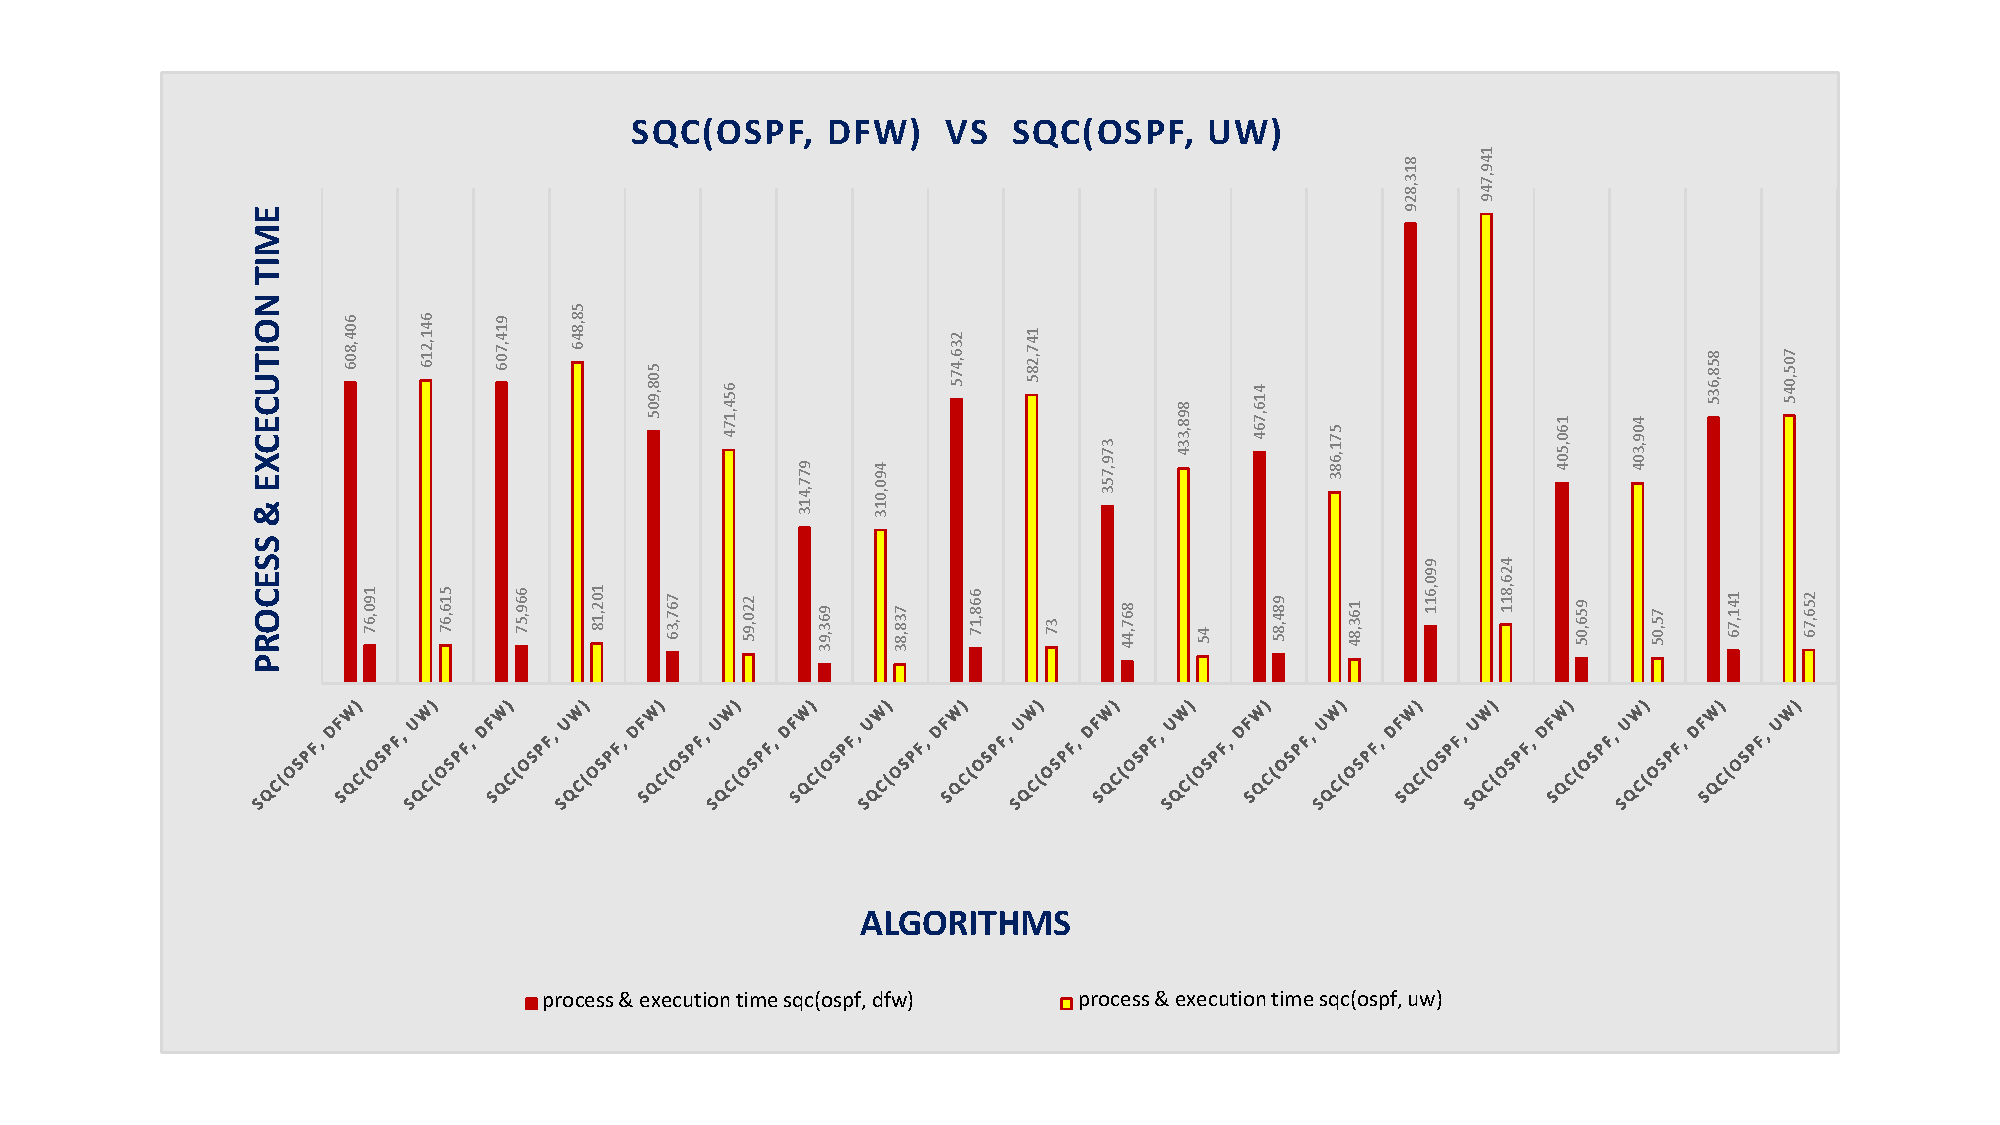
\includegraphics[width=\textwidth]{images/naveed_12.pdf}
\end{center}
\end{frame}
\begin{frame}{Ergebnisse}
\begin{center}
    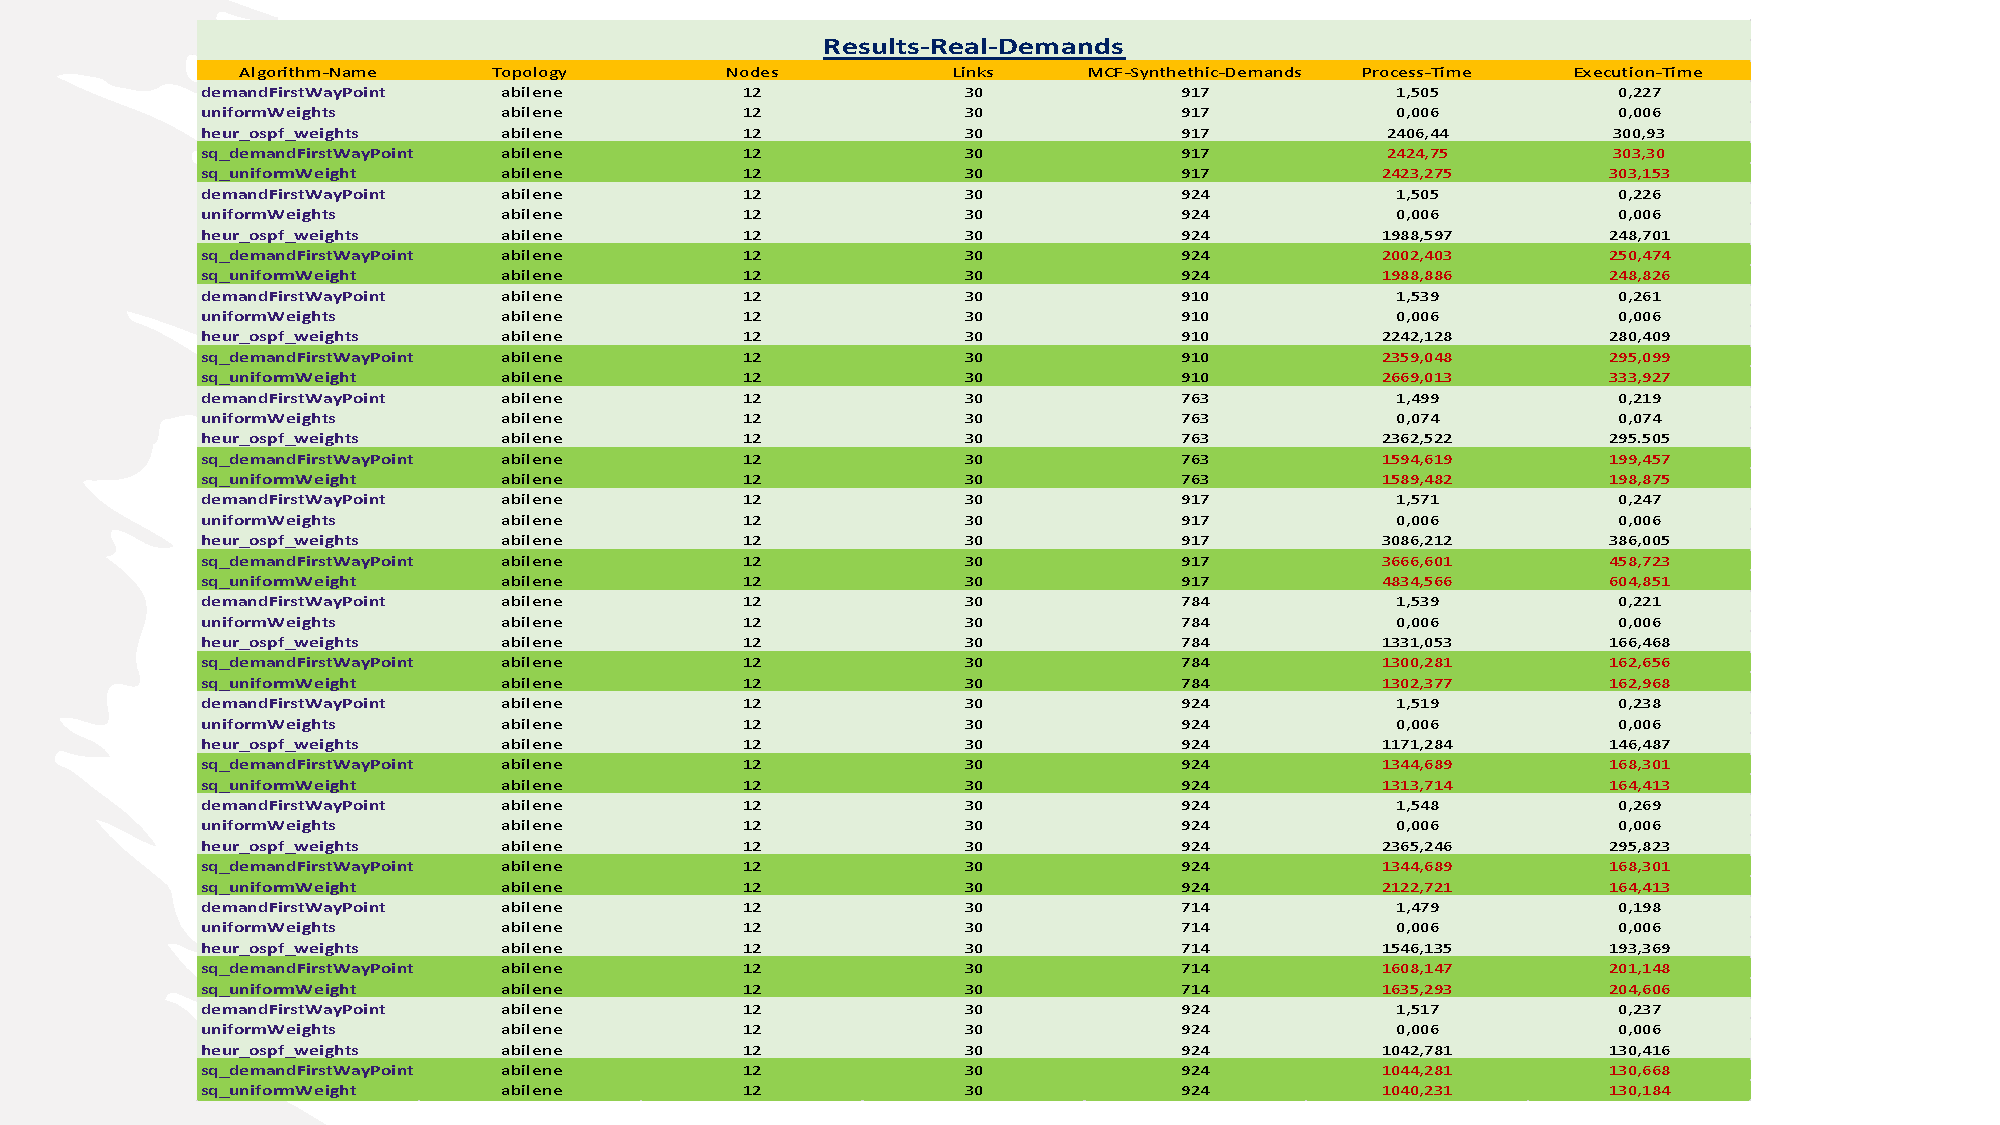
\includegraphics[width=\textwidth]{images/naveed_13.pdf}
\end{center}
\end{frame}
\begin{frame}{Ergebnisse}
\begin{center}
    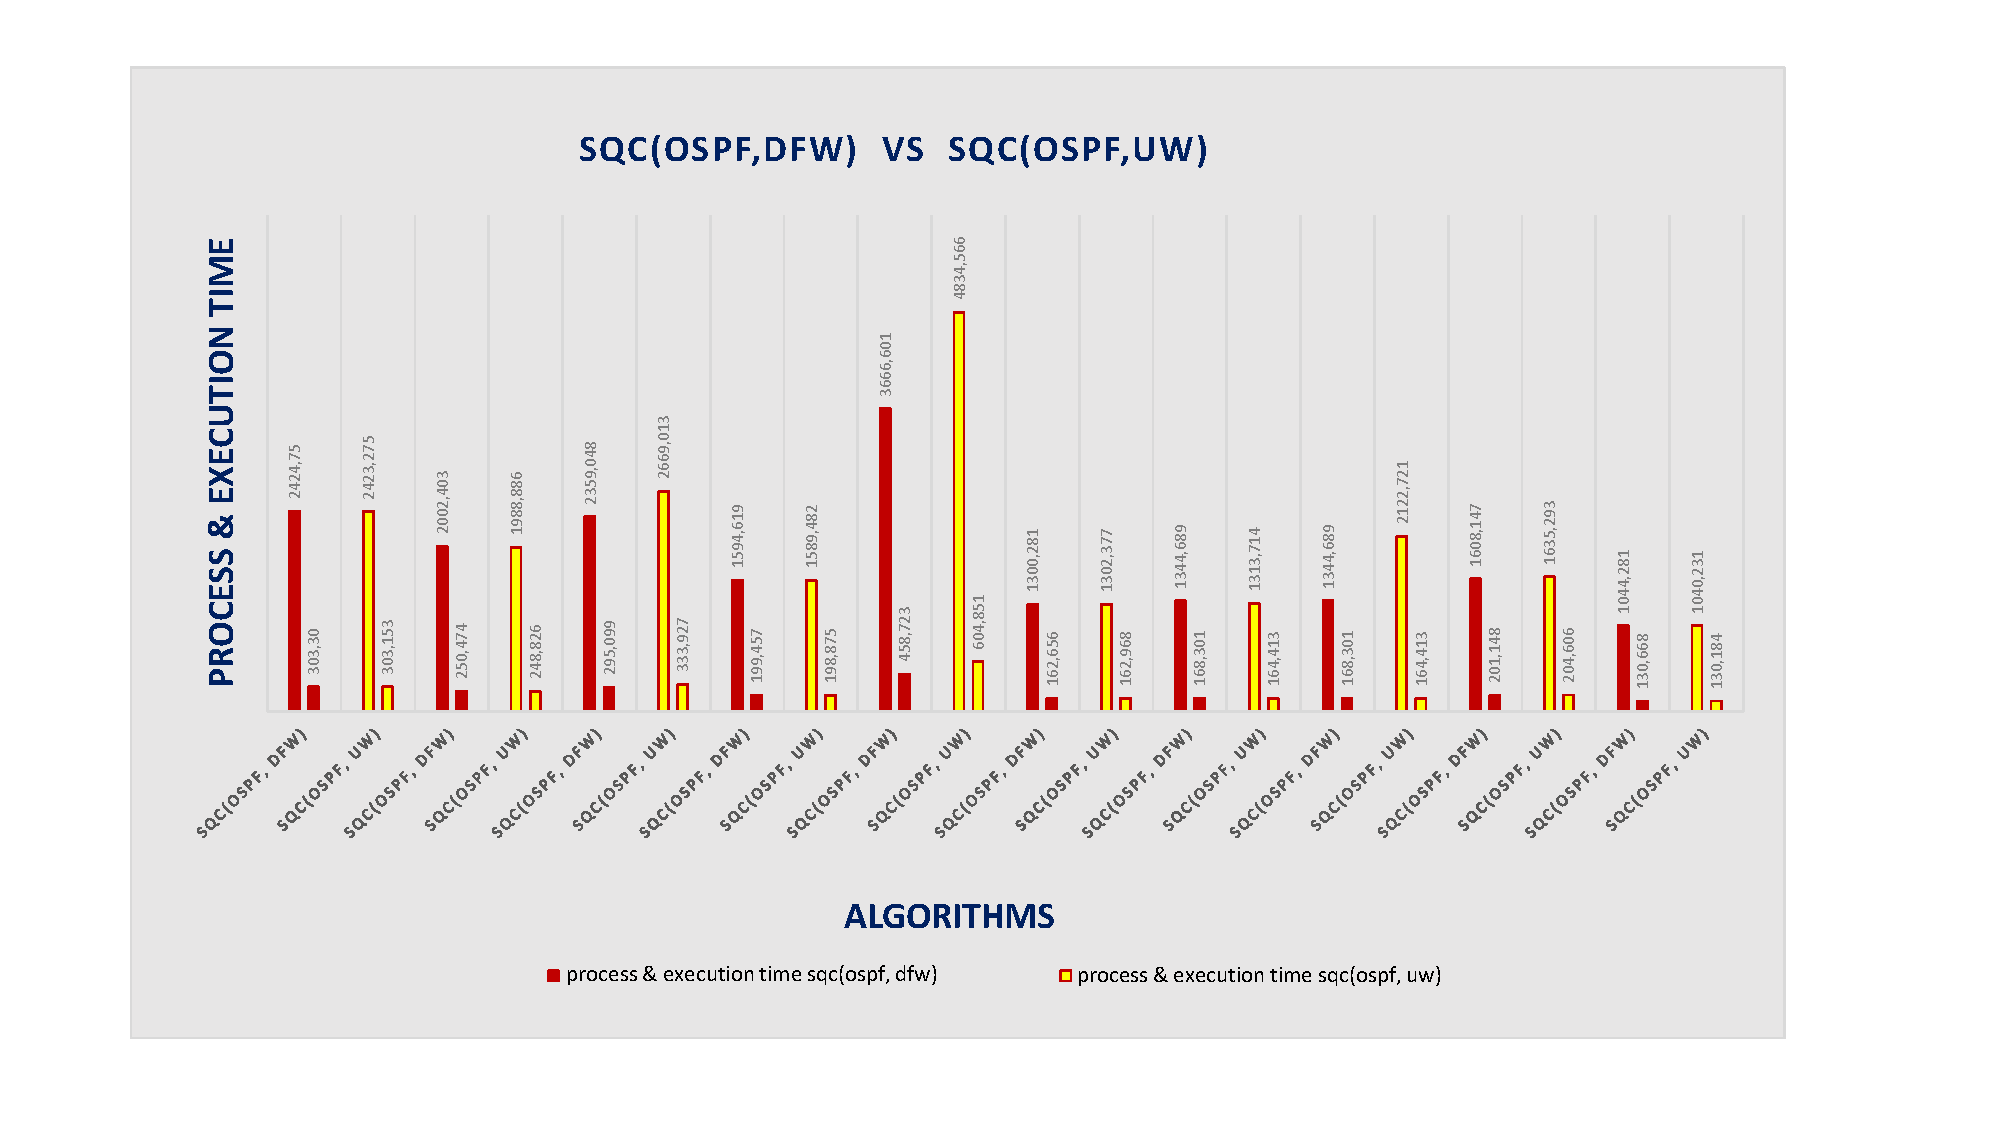
\includegraphics[width=\textwidth]{images/naveed_14.pdf}
\end{center}
\end{frame}
\begin{frame}{Ergebnisse}
\begin{center}
    
\includegraphics[width=\textwidth]{images/naveed_15.pdf}
\end{center}
\end{frame}

% %%%%%%%%%%%%%%%%%%%%%%%%%%%%%%%%%%%%%%%%%%%%%%%%
% Pouria
% %%%%%%%%%%%%%%%%%%%%%%%%%%%%%%%%%%%%%%%%%%%%%%%%

% %%%%%%%%%%%%%%%%%%%%%%%%%%%%%%%%%%%%%%%%%%%%%%%%%%%
% %%%%%%%%%%%%%%%%%%%%%%%%%%%%%%%%%%%%%%%%%%%%%%%%%%%
% Pouria
% %%%%%%%%%%%%%%%%%%%%%%%%%%%%%%%%%%%%%%%%%%%%%%%%%%%
% %%%%%%%%%%%%%%%%%%%%%%%%%%%%%%%%%%%%%%%%%%%%%%%%%%%
\section{Sequential Combination aus InverseCapacity und DemandFirstWaypoints}
% %%%%%%%%%%%%%%%%%%%%%%%%%%%%%%%%%%%%%%%%%%%%%%%%
% erste Folie
% %%%%%%%%%%%%%%%%%%%%%%%%%%%%%%%%%%%%%%%%%%%%%%%%
% zweite Folie
% %%%%%%%%%%%%%%%%%%%%%%%%%%%%%%%%%%%%%%%%%%%%%%%%
% dritte Folie
\begin{frame}{Zweiter Schritt: Motivation}
\Large
\begin{itemize}
    \item wenig Rechenzeit f\"ur $inverse\_capacity$ und $demand\_first\_waypoints$
    \item Kombi aus beidem genauer?
    \item zus\"atzliche Rechenzeit gerechtfertigt?
\end{itemize}
\end{frame}
% %%%%%%%%%%%%%%%%%%%%%%%%%%%%%%%%%%%%%%%%%%%%%%%%
% neue Folien
% %%%%%%%%%%%%%%%%%%%%%%%%%%%%%%%%%%%%%%%%%%%%%%%%
\begin{frame}{MCF Synthetic Demands}
\begin{columns}
\begin{column}{0.5\paperwidth}
\begin{center}
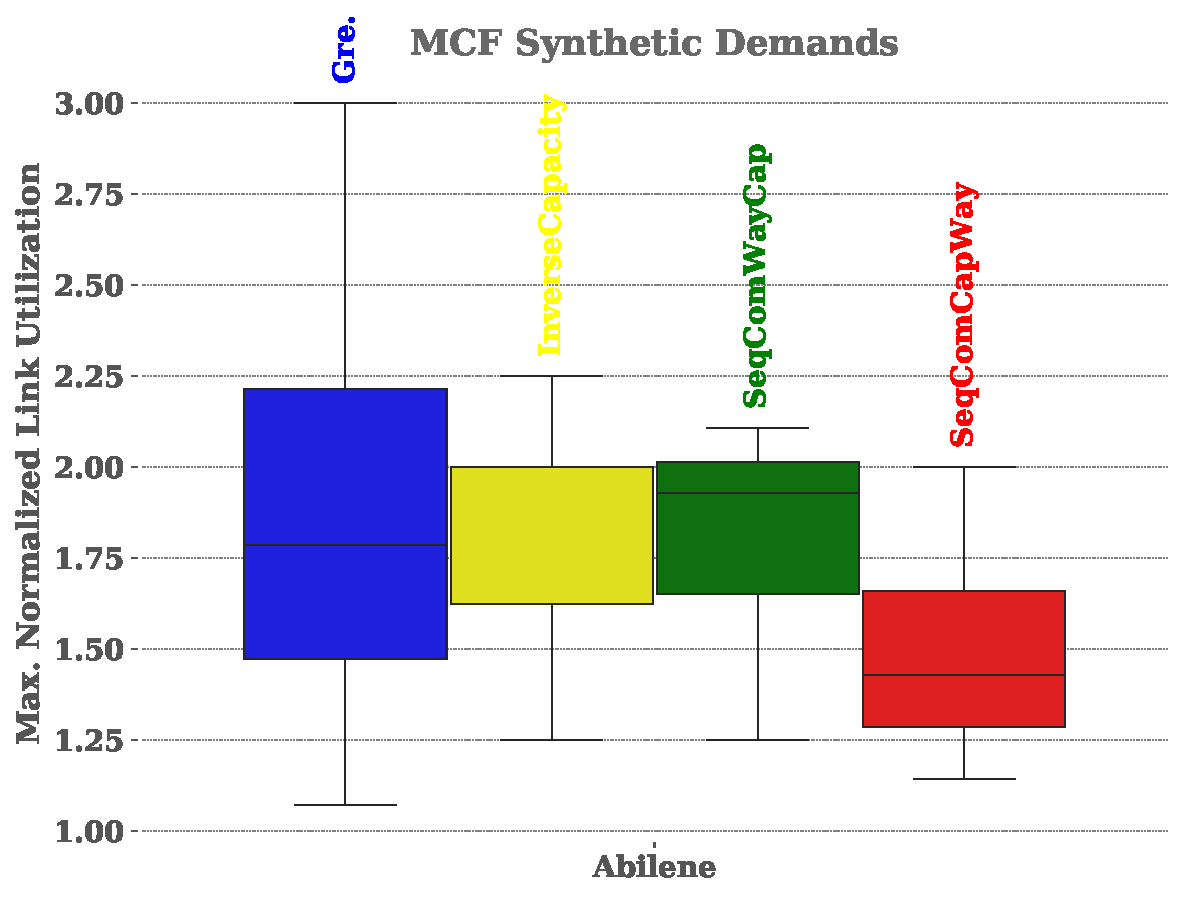
\includegraphics[width=\textwidth]{images/pouria_all_algorithms_abilene.pdf}
\end{center}
\end{column}
\hfill
\begin{column}{0.5\paperwidth}
\begin{center}
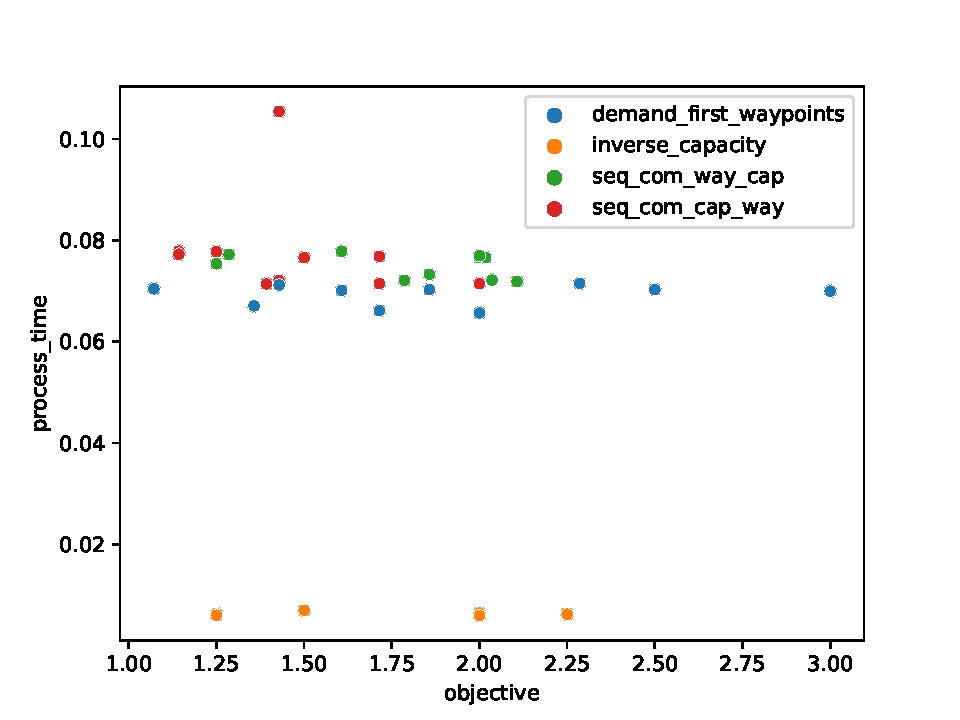
\includegraphics[width=\textwidth]{images/pouria_colored_scatter_plot_results_all_algorithms.pdf}
\end{center}
\end{column}
\end{columns}
\end{frame}
\begin{frame}{Scaled Real Demands}
\begin{columns}
\begin{column}{0.5\paperwidth}
\begin{center}
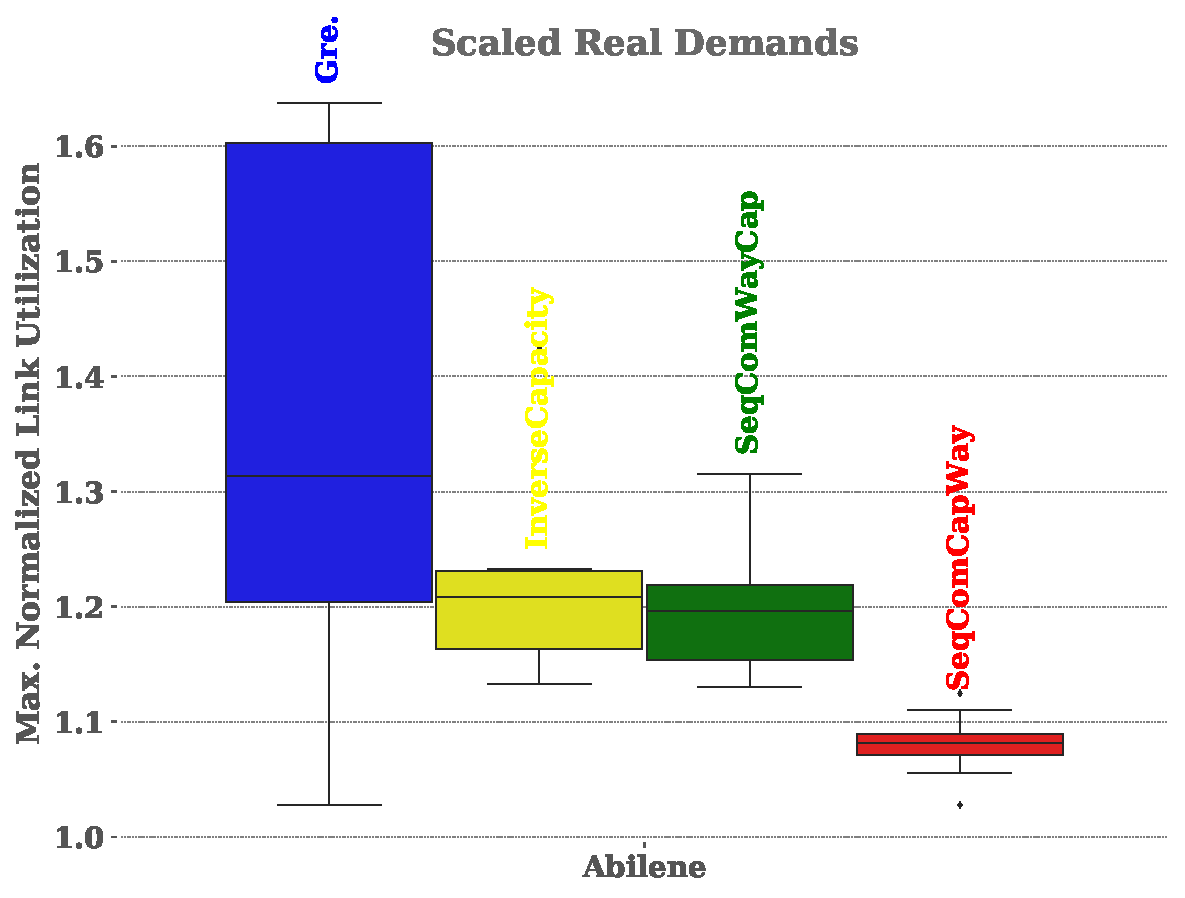
\includegraphics[width=\textwidth]{images/pouria_real_demands.pdf}
\end{center}
\end{column}
\hfill
\begin{column}{0.5\paperwidth}
\begin{center}
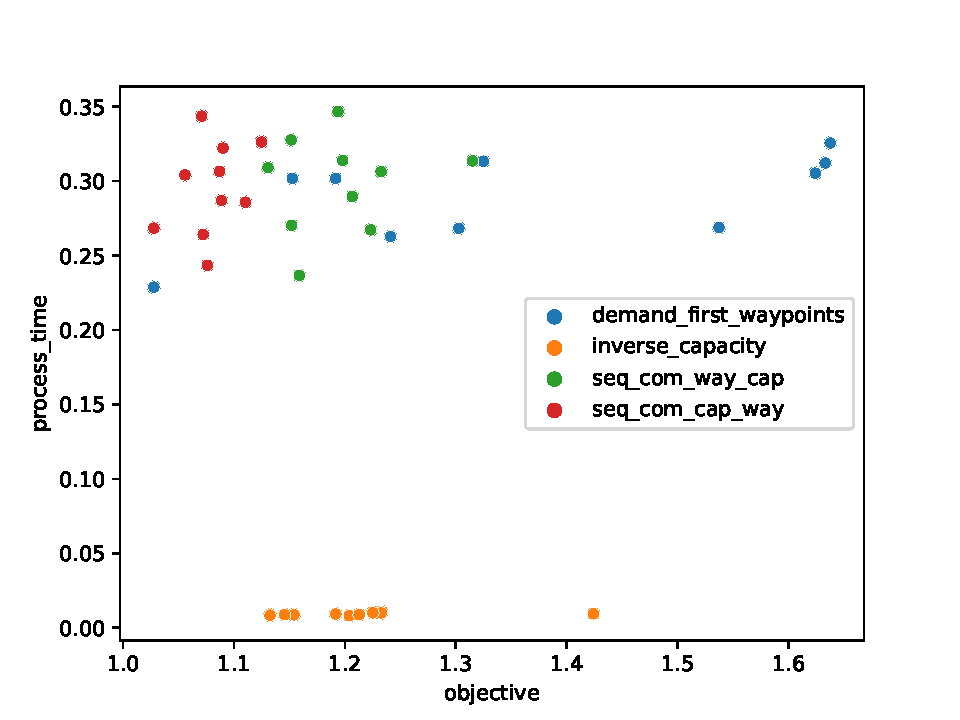
\includegraphics[width=\textwidth]{images/pouria_colored_scatter_plot_results_real_demands.pdf}
\end{center}
\end{column}
\end{columns}
\end{frame}
% %%%%%%%%%%%%%%%%%%%%%%%%%%%%%%%%%%%%%%%%%%%%%%%%
% neue Folien
% %%%%%%%%%%%%%%%%%%%%%%%%%%%%%%%%%%%%%%%%%%%%%%%%
\begin{frame}{Zweiter Schritt: Fragen}
\Large
\begin{itemize}
    \item Rechenaufwand von beiden gleich? $\rightarrow$ ja (vergleichbar)
    \item warum ist $SQ_{CW}$ besser als $SQ_{WC}$?
    \begin{itemize}
    \Large
        \item $inverse\_capacity$ bei \textcolor{green}{SeqComWayCap} versaut vorher optimierte Gewichte
        \item $inverse\_capacity$ bei \textcolor{red}{SeqComCapWay} stellt n\"utzliche Gewichte
        \item $demand\_first\_waypoints$ legt beste Route und verbessert weiter
    \end{itemize}
\end{itemize}
\end{frame}

% %%%%%%%%%%%%%%%%%%%%%%%%%%%%%%%%%%%%%%%%%%%%%%%%%%%
% %%%%%%%%%%%%%%%%%%%%%%%%%%%%%%%%%%%%%%%%%%%%%%%%%%%
% Reproduktion
% %%%%%%%%%%%%%%%%%%%%%%%%%%%%%%%%%%%%%%%%%%%%%%%%%%%
% %%%%%%%%%%%%%%%%%%%%%%%%%%%%%%%%%%%%%%%%%%%%%%%%%%%
\section{Ergebnisse Reproduktion von Gruppe 3}
\begin{frame}{main: process killed itself}
\begin{center}
    %\includegraphics[width=\textwidth]{images/err5.png}
\end{center}
\end{frame}
\begin{frame}{zixiang gu: Plottererror}
\begin{center}
    %\includegraphics[width=\textwidth]{images/err3.png}
\end{center}
\end{frame}
\begin{frame}{zixiang gu: Plottererror nach Anpassung}
\begin{center}
    %\includegraphics[width=\textwidth]{images/err1.png}
\end{center}
\end{frame}
\begin{frame}{daniel: Process killed itself}
\begin{center}
    %\includegraphics[width=\textwidth]{images/err2.png}
\end{center}
\end{frame}
\begin{frame}{daniel: Dependency nicht in README}
\begin{center}
    %\includegraphics[width=\textwidth]{images/err4.png}
\end{center}
\end{frame}

\begin{frame}[t,standout]
\Large
Fragen oder Anmerkungen?
\end{frame}
\end{document}

